\begin{refsection}
\chapter{Quantifying the relative contributions of environmental fluctuations to the maintenance of a sexually antagonistic polymorphism} % Main chapter title
\label{Coexistence_alleles}


\noindent Alba Cervantes-Loreto\textsuperscript{1},Michelle L.\ Maraffini\textsuperscript{1},Sarah P.\ Flanagan\textsuperscript{1},Daniel B.\ Stouffer\textsuperscript{1}

\begin{enumerate}
    \item Centre for Integrative Ecology, School of Biological Sciences, University of Canterbury, New Zealand
\end{enumerate}



\section*{Abstract}



Sexually antagonistic selection occurs when the direction of selection on traits or loci differs between the sexes. Sexually antagonistic selection can maintain disadvantageous alleles in a population, which underpins it's importance in maintaining polymorphism in populations with separate sexes. Importantly, theoretical studies have shown that the balancing effect of sexually antagonistic selection can increase with environmental fluctuations. Nonetheless, the quantification of the contributions of environmental fluctuations to the maintenance of polymorphism remains unknown. Thus, here we explicitly quantify the contributions of temporal fluctuations in population sizes and selection to the polymorphism of sexually antagonistic alleles. We do so by adopting an ecological framework that quantifies the relative contributions of environmental fluctuations to species growth rates when rare by using simulations. We perform simulations of alleles invading a population while allowing selection and populations sizes to fluctuate over time. Then, we used  a \textit{functional decomposition} approach to quantify the relative importance of fluctuations across the selection parameter space. Our results showed that fluctuations in selection agaisnt one allele contributed positively to the growth rate of the other allele as an invader. In contrast, fluctuations in population sizes contributed positively to alleles growth rates when rare only when alleles invaded via the fluctuating population. Finally, our results showed the importance of the correlation between fluctuations, as positively correlated fluctuations in selection but negatively correlated fluctuations in population sizes promoted the maintenance of polymorphism. Our study highlights the importance of identifying exactly how environmental drivers contribute to maintaining levels of diversity.

\section*{Introduction}
The question of how genetic variation is maintained despite the effects of selection and drift is central within evolutionary biology \citep{walsh_evolution_2018}. Classical explanations include overdominance (heterozygote advantage) or frequency-dependent selection \citep{hedrick2007balancing}, but in the modern era of genomic data, all patterns of variation that exceed the expected variation under neutrality tend to be categorized broadly as balancing selection, regardless of the evolutionary mechanism \citep{mitchell-olds_which_2007}. In species with separate sexes, balancing selection can arise due to sexually antagonistic selection \citep{connallon2014balancing}, which occurs when the direction of natural selection on traits or loci differs between the sexes \citep{lande1980sexual,arnqvist2013sexual}.

Sexually antagonistic selection can maintain genetic variation in a population \citep{chippindale2001negative,gavrilets2014sexual}, which in turn can result in phenotypically distinct sexes that express different morphological, physiological, and behavioral traits \citep{mori2017sexual,connallon2018environmental}. Nonetheless,
the extent to which sexually antagonistic selection can maintain polymorphism in a population is thought to be limited \citep{connallon2012general,connallon2018environmental}. This is because theoretical studies have found that the necessary parameter conditions that give rise to balancing selection are often highly restrictive \citep{kidwell1977regions,pamilo1979genic,hedrick1999antagonistic,curtsinger1994antagonistic}. Importantly, the effect of sexually antagonistic selection generally has been studied under strong simplifying assumptions such as constant population sizes and homogeneous environments  \citep{kidwell1977regions, pamilo1979genic, immler2012ploidally}. Studies that have explored the effect of sexually antagonistic selection with more realistic assumptions, such as temporal fluctuations in selection \citep{connallon2018environmental} or demographic fluctuations \citep{connallon2012general} have found that polymorphism can be maintained in a much wider set of conditions than classical studies predict. These results suggest that environmental fluctuations are essential to fully understand the effects of sexually antagonistic selection.

The contribution of environmental fluctuations to genetic diversity remains a debated issue in evolutionary biology. Classic theoretical models predict that temporal fluctuations in environmental conditions are unlikely to maintain a genetic polymorphism in haploid populations \citep{dempster1955maintenance,hedrick1974genetic,hedrick1986genetic}. However, other studies have found that fluctuating selection can maintain genetic variance when populations experience density dependence \citep{dean2005protecting}, overlapping generations \citep{ellner1994role, ellner1996patterns}, or when selection occurs on sex-linked traits \citep{reinhold2000maintenance}. Similarly, temporal changes in population sizes have been shown to aid in the maintenance of genetic variance \citep{whitlock1992temporal} and to mitigate the effect of genetic drift \citep{pemberton1996maintenance,nunney2002effective}. Importantly, progress requires more than just identifying \textit{if} environmental fluctuations can maintain genetic diversity in a population, but to quantify \textit{how} exactly they contribute to its maintenance \citep{ellner2016quantify}.

The mechanisms by which environmental fluctuations promote diversity maintenance have been thoroughly studied in ecological contexts \citep{levins1979coexistence,armstrong1980competitive,chesson2000mechanisms,barabas_chessons_2018}. From an ecological perspective, polymorphism of sexually antagonistic alleles is equivalent to the coexistence of species, and the fixation of one allele in a population is equivalent to competitive exclusion. Allelic polymorphism can thus be examined through the same lens as the coexistence of competing species \citep{ellner1994role,ellner1996patterns,dean2005protecting,schreiber2010interactive}. A benefit of analyzing evolutionary dynamics through this lens is that the main theoretical framework used to examine how competing species coexist, Modern Coexistence Theory \citep{chesson2000mechanisms, barabas_chessons_2018}, allows the explicit quantification of how environmental fluctuations contribute to coexistence.

Modern Coexistence Theory posits that coexistence is promoted by processes that give any species, when rare, an advantage over the existing species in a community \citep{chesson_multispecies_1994,chesson2000mechanisms}. Environmental fluctuations can give species advantages when rare if competitors respond differently to limiting competitive factors, a mechanism known as \textit{relative non-linearity} \citep{chesson2000mechanisms,ellner2016quantify,zepeda2019fluctuation}. Differential responses to environmental fluctuations can further give species advantages when rare if fluctuations in environmental factors covary with competitive factors and species are less sensitive to competition in good environmental conditions, a mechanism known as the \textit{the storage effect} \citep{chesson2000mechanisms,ellner2016quantify,barabas_chessons_2018,schreiber2021positively}. This list is not exclusive, as there are a plethora of ways in which environmental heterogeneity can give species advantages when rare \citep{ellner_expanded_2019}. Nonetheless, there is no study to our knowledge that directly quantifies how environmental fluctuations contribute to the maintenance of a sexually antagonistic polymorphism under the lens of Modern Coexistence Theory.

%Despite that an exact correspondence to MCT is probably unattainable,

The use of Modern Coexistence Theory historically required complex mathematical analysis of the models describing the systems dynamics and restrictive assumptions \citep{barabas_chessons_2018}; however, recent computational approaches allow the quantification of the relative importance of environmental fluctuations to coexistence using simulations \citep{ellner2016quantify,ellner_expanded_2019,shoemaker2020}. Here, we seek to explicitly quantify how temporal environmental fluctuations contribute to the maintenance of polymorphism under sexually antagonistic selection by applying recent advances in Modern Coexistence Theory.  We examined how fluctuations in selection, fluctuations in population sizes, and its interaction can further or hinder the maintenance of polymorphism. In particular, we examined i) Can fluctuations in population sizes and selection allow sexually antagonistic alleles to coexist when differences in their fitness would typically not allow them to? and ii) What are the relative contributions of different types of fluctuations that allow or impede two sexually antagonistic alleles to be maintained in a population? Our study provides the tools to analyze sexual antagonism from a novel perspective and contributes to answering long-lasting questions regarding the effect of non-constant environments on genetic diversity.


\section*{Methods}

We first present a model that describes the evolutionary dynamics of sexually antagonistic alleles. We then show how we simulated different scenarios of alleles invading a population, where we allowed selection, population sizes, both, or neither to vary. Finally, we detail how we examined the relative contribution of each type of fluctuation to the maintenance or loss of polymorphism.

\subsection*{Population dynamics of sexually antagonistic alleles}


Our model examines evolution at a single, biallelic locus. We further assum the relative fitness of each allele was frequency and density independent. We examine the dynammics of two  sexually antagonistic alleles, $j$ and $k$, that affect fitness in the haploid state. The frequencies of each allele in each sex at the beginning of a life-cycle at generation $t$ are given by:
\begin{equation}
    p_{jm,t}= \frac{n_{jm,t}}{N_{m,t}}
    \label{first_pop}
\end{equation}
\begin{equation}
    p_{jf,t}= \frac{n_{jf,t}}{N_{f,t}}
\end{equation}
\begin{equation}
    p_{km,t}=  \frac{N_{m,t}-n_{jm,t}}{N_{m,t}}
\end{equation}
\begin{equation}
    p_{kf,t}= \frac{N_{f,t}-n_{jf,t}}{N_{f,t}}
\end{equation}
where $N_{m,t}$ and $N_{f,t}$ are the total numbers of males and females in the population at generation $t$, respectively, while $n_{jf,t}$ is the number of females $f$ with allele $j$, and $n_{jm,t}$ is the number of males $m$ with allele $j$ at time $t$. Since the locus is biallelic, the number of males with allele $k$ at generation $t$ is given by $n_{km,t}=N_{m,t}-n_{jm,t}$ and the number of females with allele $k$ by $n_{kf,t}=N_{f,t}-n_{jf,t}$.

The individuals in the population mate at random before selection occurs, and therefore the frequency of offspring with allele $j$ after mating, $p'_{j,t}$ can be expressed as:
\begin{equation}
   p'_{j,t}= \frac{n_{jf,t}}{N_{f,t}} \frac{n_{jm,t}}{N_{m,t}} + \frac{1}{2} \frac{n_{jf,t}}{N_{f,t}} \frac{(N_{m,t}-n_{jm,t})}{N_{m,t}} +\frac{1}{2}
   \frac{(N_{f,t}-n_{jf,t})}{N_{f,t}} \frac{n_{jm,t}}{N_{m,t}}
   \label{prime_a}
\end{equation}
which upon rearranging and simplifying gives:
\begin{equation}
   p'_{j,t}= \frac{N_{m,t}n_{jf,t}+ N_{f,t}n_{jm,t}}{2 N_{f,t}N_{m,t}}
   \label{pprime}
\end{equation}

To illustrate how allele frequencies change through time, we use allele $j$ as an example. However, an equivalent expression for allele $k$ can be obtained by interchanging $k$ subscripts for $j$ in Eqn.~\ref{pprime}. Selection acts upon these offspring in order to determine the allelic frequencies in females and males in the generation $t+1$. As an example, the frequency  of females with allele $j$ after selection is given by:
\begin{equation}
   p_{jf, t+1}= \frac{n_{jf, t+1}}{N_{f,t+1}} = \frac{p'_{j,t}w_{jf}}{p'_{t,j}w_{jf}+ (1-p'_{t,j})w_{kf}}
   \label{next_gen}
\end{equation}
Changes in alleles frequencies can also be expressed in terms of growth rates, which is useful to consider when doing analysis under Modern Coexistence Theory. The logarithmic per capita growth rate of allele $j$ in females is given by the number of females carrying allele $j$ after selection divided by the original number of females carrying allele $j$:
\begin{equation}
    r_{jf,t} = \ln \left( \frac{n_{jf, t+1}}{n_{jf,t}} \right)
    \label{canonical}
\end{equation}
An equivalent expression for the logarithmic per capita growth rate of allele $j$ in males $m$ can be obtained by exchanging $f$ for $m$ across the various subscripts in Eqn.~\ref{canonical}. Polymorphism in a sexual population, however, is ultimately influenced by growth and establishment of an allele across both sexes. Therefore, the growth rate of allele $j$ across the entire population of females \emph{and} males is given by:
\begin{equation}
    r_{j,t} = \ln \left( \frac{n_{jf, t+1} + n_{jm, t+1} }{n_{jf,t} + n_{jf,t} }  \right)
    \label{full}
\end{equation}
An equivalent expression describes $r_{k,t}$, the growth rate of allele $k$.


Our model further assumed allele $j$ always has a high fitness in females ($w_{jf} = 1$) with lower fitness in males ($w_{jm} < 1$); and allele $k$ has a high fitness in males ($w_{km} = 1$)  with lower fitness in females ($w_{kf} < 1 $). The strength of selection against allele $j$ in males is therefore $S_{m}= 1 - w_{jm}$, and the strength of selection against allele $k$ in females is $S_{f}= 1 - w_{kf}$. When population sizes and selection are constant,
selection mantains both alleles in the population under the condition that:

\begin{equation}
\frac{S_{m}}{1+S_{m}} < S_{f} < \frac{S_{m}}{1-S_{m}}
\label{selection}
\end{equation}
\citep{kidwell1977regions,pamilo1979genic,patten2010fitness,connallon2018environmental}. Thus, the maintenance of polymorphism of sexually antagonistic alleles is solely determined by the values of $S_{m}$ and $S_{f}$. Note that in our model, the values $S_{m}$ and $S_{f}$ are bounded from $0$ to $1$. Therefore the parameter space of sexually antagonistic selection is within the range $ 0< S_{m}, S_{f} < 1$. Classic theoretical models predict that, in constant environments, polymorphism is maintained in $\approx 38\%$ of the parameter space \citep{kidwell1977regions,pamilo1979genic,connallon_evolutionary_2019}. Nonetheless, it is unrealistic to assume population sizes and selection are constant through time. Temporal changes in population densities are ubiquitous in nature \citep{whitlock1992temporal,connallon2012general,reinhold2000maintenance}. Similarly, the effect of sexual selection has been shown to vary through space and time \citep{kasumovic2008spatial}. If fluctuations in population sizes or selection values affect the coexistence of sexually antagonistic alleles, it should be reflected in increases or decreases of the proportion of the parameter space across which polymorphism is maintained.


\subsection*{Simulations}
We examined the effect of fluctuating population sizes and selection in the maintenance of a genetic polymorphism across the selection parameter space ($0 < S_{m}, S_{f} < 1$). To do so, we partitioned the parameter space into a $50 \times 50$ element grid, which yielded 2500 different pairwise combinations of $w_{jm}$ and $w_{kf}$ values. Henceforth, we will refer to the set of combinations of $w_{jm}$ and $w_{kf}$ values that make up the parameter space of sexually antagonistic selection as a grid. For each pairwise combination of $w_{jm}$ and $w_{kf}$, as we detail in the next sections, our simulation approach consisted of three main parts. First, we incorporated fluctuations in population sizes and selection into our population dynamics model. Second, we performed simulations to evaluate if both alleles could be maintained in a population when the environment fluctuated. Finally, we determined the relative contribution of each type of fluctuation to the maintenance of each allele.

For each grid, which was our unit of replication, we controlled the effect size of  fluctuations in selection ($\sigma_{w}$) and their correlation ($\rho_{w}$), as well as the effect size of fluctuations in population sizes ($\sigma_{g}$) and their correlation ($\rho_{g}$). We explored all of  the combinations of low, intermediate, and high fluctuations in selection and population sizes, with different extents of correlations between fluctuations (Table \ref{tab:fluctuations}).  As a control simulation, we set $\sigma_{w}=1e^{-4}$ and  $\sigma_{g}=1e^{-4}$, with no correlation between fluctuations. In total, we explored 378 parameter combinations. We ran ten replicates per parameter combination, which resulted in 3780 grids.


\begin{table}[h]
\fontsize{7}{10}\selectfont
\centering
\caption[Parameters used in our simulations to control the effect sizes of fluctuations in population sizes ($\sigma_{g}$) and selection values ($\sigma_{w}$) and their respective correlations ($\rho_{g}$ and $\rho_{w}$)]{Parameters used in our simulations to control the effect sizes of fluctuations in population sizes ($\sigma_{g}$) and selection values ($\sigma_{w}$) and their respective correlations ($\rho_{g}$ and $\rho_{w}$). We ran ten replicates for each of the factorial combinations of the following parameters, which yielded a total of grids. }
\begin{tabular}{@{}llll@{}}
\toprule
Parameter                    & Values                    & Description                                   &  \\ \midrule
$\sigma_{w}$ & 0.0001, 0.1, 0.3, 0.5, 0.7, 0.9 & Effect size of fluctuations in fitness values &  \\
$\sigma_{g}$ & 0.0001, 10, 20, 30, 50, 70 & Effect size of fluctuations in population sizes                                              &  \\
$\rho_{w}$  &  -0.75, 0, 0.75                         &   Correlation between fluctuations in fitness values                                            &  \\
$\rho_{g}$  &   -0.75, 0, 0.75                        &  Correlation between fluctuation in population sizes                                             &  \\ \bottomrule
\end{tabular}
\label{tab:fluctuations}
\end{table}
%We explored all of  the combinations of low ($\sigma_{w}\in{(0.1, 0.3)}$, $\sigma_{g}\in{(1,10)}$), intermediate ($\sigma_{w}\in{(0.5, 0.7)}$, $\sigma_{g}\in{(20,30,50)}$), and high fluctuations ($\sigma_{w}= 0.9$, $\sigma_{g}=70$)  in selection and population sizes, with different extents of correlations between fluctuations (Table \ref{tab:fluctuations})
\subsubsection*{Environmental timeseries}

To incorporate the effects of fluctuations into our population dynamics model, we generated independent timeseries of fluctuations in selection and population sizes. In the case of fluctuations in selection values, for a given value of $w_{jm}$ and $w_{kf}$ (i.e., a fixed point in the parameter space), we generated a timeseries of 500 generations made up of correlated fluctuations of $w_{jm}$ and $w_{kf}$. We controlled the size of  fluctuations in selection ($\sigma_{w}$) and correlation between sexes ($\rho_{w}$) by  using the variance-covariance matrix:

\begin{equation}
C_{w} = \begin{bmatrix}
\sigma_{w}^{2} & \rho_{w} \sigma_{w}^{2} \\
\rho_{w} \sigma_{w}^{2} & \sigma_{w}^{2}
\end{bmatrix}
\label{covmat}
\end{equation}

We then performed a Cholesky decomposition of $C_{w}$ and multiplied it by a $2 \times 500$ matrix of random uncorrelated numbers from a unit normal distribution, which yielded  $\gamma_{j,t}$ and $\gamma_{k,t}$. Since fitness values are bounded from zero to one, we transformed fitness values as $w'_{jm} = \ln\frac{w_{jm}}{1-w_{jm}}$ and $w'_{kf} = \ln\frac{w_{kf}}{1-w_{kf}}$. Finally, we calculated the fitness values at generation $t$ as:

\begin{eqnarray}
  w_{jm,t}= \frac{e^{(w'_{jm}+ \gamma_{j,t})}}{1+ e^{(w'_{jm}+ \gamma_{j,t})}} \\
    w_{kf,t}= \frac{e^{(w'_{kf}+ \gamma_{k,t})}}{1+ e^{(w'_{kf}+ \gamma_{k,t})}}
    \label{logistic_w}
\end{eqnarray}
This approach guaranteed that fluctuations in $w_{jm}$ and $w_{kf}$ were always bounded from zero to one.

Similarly, we generated an independent timeseries of 499 generations made up of correlated fluctuations in population sizes. Note, that in contrast to fluctuations in selection, we controlled the initial values of the timeseries by setting the male and female populations at 200 individuals each ($N_{m,0} =200$ and $N_{f,0} =200$). Then, we used the Cholesky factorization of the variance-covariance matrix to control the size of fluctuations in population sizes with $\sigma_{g}$ and their correlation with $\rho_{g}$. Similar to our previous approach, we multiplied this factorization by a $2 \times 499$ matrix of random uncorrelated numbers from a unit normal distribution, which yielded $\gamma_{m,t}$ and $\gamma_{f,t}$. We calculated the number of males and females in the population at generation $t$ as $N_{m,t} = N_{m,0} + \gamma_{m,t}$ and $N_{f,t} = N_{f,0}+ \gamma_{f,t} $. Therefore, the population sizes in each generation differed from the initial value of 200 individuals on the order of $\sigma_{g}$. To avoid extinction due to fluctuations in population sizes, we imposed a lower bound of one individual on the population sizes of both sexes. Note that the scales of $\sigma_{g}$ and  $\sigma_{w}$ are different from each other. While $\sigma_{w}$ controls the change in fitness values in logistic space, $\sigma_{g}$ controls the number of individuals added or removed from the initial population.

%We bounded the values population sizes could take so there were no negative population sizes since that would not be biologically plausible. We did not impose an upper bound to the values population sizes could take.

%We chose values of $N_{m}= 200$ and $N_{f}=200$ as the initial value of population sizes throughout our simulations.

Finally, we performed simulations where our population dynamics model (Eqns.~\ref{first_pop} to \ref{full}) was iterated over 500 generations while selection and population sizes fluctuated in each generation. We started each simulation with initial values of 200 individuals of males and females and equal frequencies of allele $j$ and allele $k$ in each sex. For each generation $t$ in our simulations, the values of $w_{jm,t}$ $w_{kf,t}$, $N_{m,t}$ and $N_{f,t}$ used to calculate allele frequencies in generation $t$ (e.g., Eqn.~\ref{next_gen}), corresponded to the values at generation $t$ calculated in the corresponding timeseries, as described previously. This approach yielded a final timeseries that captured the dynamics of sexually antagonistic alleles with fluctuating values of selection and population sizes.

\subsubsection*{Invasion simulations}

 To evaluate if both alleles could be maintained in a population when the environment fluctuated, we turned towards Modern Coexistence Theory. Modern Coexistence Theory has shown that coexistence is promoted by mechanisms that give a species when rare, a population growth rate advantage over other species \citep{chesson_multispecies_1994,chesson2000mechanisms, barabas_chessons_2018}. To test this idea, one species is held at its \textit{resident} state, as given by its steady-state abundance, while the rare species is called the \textit{invader}. In the context of alleles in a population, an allele is an \textit{invader} when a mutation occurs that introduces that allele into a population in which it is absent (e.g., in a population with only $k$ alleles, if a random mutation leads to one individual carrying the $j$ allele). Within a sexual population, each allele has two pathways of invasion, depending on whether the mutation arises in a female or in a male. If an allele's \textit{invasion growth rate} (or the average per capita logarithmic growth rate when rare) is positive, it buffers it against extinction, maintaining its persistence in the population.  Coexistence, and hence polymorphism, occurs when both alleles have positive invasion growth rates.

We used the timeseries that captured the dynamics of our population model with environmental fluctuations as a template to perform invasion simulations of both alleles. Following the approach of \citet{ellner2016quantify}, we treated each invasion simulation independently, and hence we performed 500 invasion simulations, one for each generation in our timeseries. We explored all four potential combinations of each allele ``invading'' through each sex (e.g., allele $j$ invading through males, allele $k$ invading through females, and so on). To simulate invasion, we set the numbers of individuals carrying the invading allele to one individual. Since we treated each invasion simulation as an independent event, we denoted the initial timestep in an invasion simulation with the subscript $i$. For example, if allele $j$ was invading via males, then we would set $n_{jm,i} = 1$ and $n_{jf,i}= 0$. We also set the resident allele, in this case $k$, to the corresponding population size of the timeseries minus the one invading individual, $n_{km,i} = N_{m,t} -1$ and $n_{kf,i} = N_{f,t}$. We then simulated invasion by simulating one generation of our population dynamics model (i.e., to generate $i+1$) and calculated the logarithmic growth rate of the invading allele according to Eqn.~\ref{full}, which in this example would be given by:
 %We allowed each allele to invade via two different pathways: males and females
%For each timestep in the timeseries, we performed simulations of the two alleles invading separately via their respective pathway.


\begin{equation}
r_{j,i} =	\ln \left ( \frac{n_{jm,i+1 } + n_{jf,i+1}}{1} \right )
\label{invader}
\end{equation}
Similarly, the logarithmic growth rate of the resident allele would be given by:
\begin{equation}
r_{k,i} =	\ln \left ( \frac{ n_{km,i+1} + n_{kf,i+1} }{ n_{km,i} + n_{kf,i}  } \right )
\label{resident}
\end{equation}
We then calculated the mean logarithmic growth rate of each allele as an invader as the average of the 500 invasion growth rates. We also calculated the mean logarithmic growth rate of each allele as a resident as the average of the 500 resident growth rates. We determined alleles could coexist  and therefore polymorphism could be maintained when both alleles had positive mean invasion growth rates, which is often referred to as the mutual invasibility criterion \citep{barabas_chessons_2018}.


\subsubsection*{Functional decomposition}


Our invasion simulations allows us to evaluate whether or not polymorphism can be maintained at a given point of the parameter space with and without environmental fluctuations. However, we also quantify the relative contributions of fluctuations in selection and population sizes to the predicted coexistence outcome using a \textit{functional decomposition} approach \citep{ellner2016quantify,ellner_expanded_2019, shoemaker2020}. This approach allows the quantification of processes affecting growth rates in an analogous way, but not limited to, the mechanisms proposed by Modern Coexistence Theory \citep{ ellner2016quantify, ellner_expanded_2019}

%also wanted to quantify the relative contributions of fluctuating selection and population sizes into the predicted coexistence outcome. Therefore, we turned towards an extension of modern coexistence theory \citep{ellner_expanded_2019} that provides the flexibility to analyze the contributions of different processes to coexistence using \textit{functional decomposition}. This approach applies to any collection of two or more processes, mechanisms, or species differences affecting population growth rate \citep{ ellner2016quantify, ellner_expanded_2019}, and has been used to show the relative contribution of variable temperature and silicate to the coexistence of algal species \citep{ellner2016quantify} and to quantify the relative importance of environmental fluctuations and variation in predator abundances to the coexistence of intertidal species \citep{shoemaker2020}.


%Modern coexistence theory provides an analytical framework to decompose each allele´s, invasion growth rates into a sum of terms for the effects of different factors, such as abiotic and biotic fluctuations, and then compare invader and residents term by term \citep{ellner_expanded_2019}. Mechanisms that promote coexistence can help whichever allele is rare, or it can hurt whichever allele is common. Therefore, to understand the role of each mechanism, it is necessary to compare how it affects invader \textit{and} resident growth rates.

%modern coexistence theory uses Taylor series expansion to do this decomposition and comparison (a detailed review can be found in \citet{barabas_chessons_2018}). We present an analytical approach, using classic modern coexistence theory, to understand the relative contributions of fluctuation in population sizes and fitness values to each alleles' growth rate as an invader in the Supporting Information.

The functional decomposition approach separates the average growth rate of each allele into a null growth rate in the absences of fluctuations in all selected variables, a set of main effect terms that represent the effect of only one variable fluctuating, a set of two-way interaction terms representing the effect of variables fluctuating simultaneously, and so on \citep{ellner_expanded_2019}. In our simulations, this is a function of four variables: the number of males in the population ($N_{m}$), the number of females in the population ($N_{f}$), the fitness of allele $j$ in males ($w_{jm}$), and the fitness of allele $k$ in females ($w_{kf}$). As a simplified example, if only $N_{m}$ and $N_{f}$ were fluctuating, the growth rate of allele $j$ as an invader (Eqn.~\ref{invader}) at generation $i$ could be decomposed into:

\begin{equation}
   r_{j,i}(N_{m},N_{f}) = \mathcal{E}_{j}^{0} + \mathcal{E}_{j}^{N_{m}}+ \mathcal{E}_{j}^{N_{f}}+ \mathcal{E}_{j}^{N_{m}N_{f}}
   \label{functional_decomp}
\end{equation}
where $\mathcal{E}^0$ is the null growth rate when $N_{m}$ and $N_{f}$ are set to their averages from the timeseries. Terms with superscripts represent the marginal effects of letting all superscripted variables vary while fixing all the other variables to their average values. For example, the term $\mathcal{E}_{j}^{N_{m}}$ expresses the contribution of fluctuations in $N_{m}$ when $N_{f}$ is set to its average, without the contribution when both variables are set to their averages:

\begin{equation}
  \mathcal{E}_{j}^{N_{m}} = r_{j,i}(N_{m},\overline{N_{f}}) - \mathcal{E}_{j}^{0}
\end{equation}
If we average Eqn.~\ref{functional_decomp} across the 500 invasion simulations, we get a partition of the average population growth rate into the variation free growth rate, the main effect of variability in $N_{m}$, the main effect of variability in $N_{f}$, and the interaction between variability in $N_{m}$ and $N_{f}$:

\begin{equation}
    \overline{r_{j}}= \mathcal{E}_{j}^{0} + \overline{\mathcal{E}_{j}}^{N_{m}}+ \overline{\mathcal{E}_{j}}^{N_{f}}+ \overline{\mathcal{E}_{j}}^{N_{m}N_{f}}
   \label{functional_decomp_2}
\end{equation}

In our simulations, $w_{jm}$ and $w_{kf}$ also fluctuate, therefore the full functional decomposition of the growth rate of allele $j$ as an invader is found in Table \ref{tab:EllnerRs}, as well as a brief description of the meaning of each term. For simplicity, we only show terms related to allele $j$ as an invader; however, the functional decomposition approach can be applied analogously when allele $k$ invades. Note that Table \ref{tab:EllnerRs} does not include three-way or four-way interactions (e.g., $\overline{\mathcal{E}_{j}}^{N_{m}N_{f}w_{jm}w_{fk}}$). This is because we did not allow fluctuations in selection and population sizes to be correlated in our simulations. Therefore their effects are fully captured by the terms in Table \ref{tab:EllnerRs}. We calculated the value of each of the terms in Table \ref{tab:EllnerRs} by performing additional sets of invasion simulations controlling which variables were allowed to fluctuate. For example, to calculate the value of $\mathcal{E}_{j}^{0}$, we performed another 500 simulations of allele $j$ invading but, instead of using the values of $w_{jm,i}$ $w_{kf,i}$, $N_{m,i}$ and $N_{f,i}$ used to simulate the frequency of allele $j$ in generation $i+1$, we set all of them to their mean value. To calculate the value of $\mathcal{E}_{j}^{N_{m}}$, we set all variables except $N_{m}$ to their mean value and subtracted the value of $\mathcal{E}_{j}^{0}$, and so on with subsequent terms.


\begin{table}[h]
\fontsize{7}{12}\selectfont % the spacing on this is rough
    \centering
      \caption{Functional decomposition of the growth rate of allele $j$. As defined in Eqn.~(\ref{functional_decomp_2}), the partition of the average population growth rate is made up of the variation free growth rate ($\mathcal{E}^{0}_{j}$), main effects of each variable fluctuating, and the interaction between fluctuations in correlated variables. }
  \resizebox{\textwidth}{!} {\begin{tabular}{l|l|l}
  \toprule
        Term & Formula & Meaning \\
        \hline
         $\mathcal{E}^{0}_{j}$ & $\overline{r_{j}} (\overline{N_{m}}, \overline{N_{f}}, \overline{w_{jm}}, \overline{w_{kf}})$ & Growth rate at mean population size and selection values \\


         $\overline{\mathcal{E}_{j}}^{N_{m}}$ & $\overline{r_{j}}(N_{m} \overline{N_{f}}, \overline{w_{jm}}, \overline{w_{kf}}) - \mathcal{E}^{0}_{j} $ & Main effect of fluctuations in $N_{m}$\\

         $\overline{\mathcal{E}_{j}}^{N_{f}}$ & $ \overline{r_{j}}( \overline{N_{m}}, N_{f},\overline{w_{jm}}, \overline{w_{kf}}) - \mathcal{E}^{0}_{j}$ & Main effect of fluctuations in $N_{f}$ \\

        $\overline{\mathcal{E}_{j}}^{w_{jm}}$ & $ \overline{r_{j}}(\overline{N_{m}}, \overline{N_{f}}, w_{jm}, \overline{w_{kf}}) - \mathcal{E}^{0}_{j}$& Main effect of fluctuations in $w_{jm}$\\

        $\overline{\mathcal{E}_{j}}^{w_{kf}}$ & $ \overline{r_{j}}(\overline{N_{m}}, \overline{N_{f}}, \overline{w_{jm}}, w_{kf})- \mathcal{E}^{0}_{j}$ & Main effect of fluctuations in $w_{kf}$\\

        $\overline{\mathcal{E}_{j}}^{N_{m},N_{f}}$ & $ \overline{r_{j}}(N_{m}, N_{f}, \overline{w_{jm}}, \overline{w_{kf}})- [\mathcal{E}^{0}_{j} +\overline{\mathcal{E}_{j}}^{N_{m}}+\overline{\mathcal{E}_{j}}^{N_{f}}]$ & Interaction effect of fluctuations in $N_{m}$ and $N_{f}$\\

        $\overline{\mathcal{E}_{j}}^{w_{jm},w_{kf}}$ & $ \overline{r_{j}}(\overline{N_{m}}, \overline{N_{f}}, w_{jm}, w_{kf})- [\mathcal{E}^{0}_{j} +\overline{\mathcal{E}_{j}}^{w_{jm}}+\overline{\mathcal{E}_{j}}^{w_{kf}}]$ & Interaction effect of fluctuations in $w_{jm}$ and $w_{kf}$ \\

      %  $\overline{\mathcal{E}}^{N_{m}w_{jm}}_{j}$ & $\overline{r_{j}}(N_{m}, \overline{N_{f}}, w_{jm}, \overline{w_{kf}})- [\mathcal{E}^{0}_{j} +\overline{\mathcal{E}}^{N_{m}}_j+\overline{\mathcal{E}}^{w_{jm}}_{j}]$  & Interaction of fluctuations in $N_{m}$ and $w_{jm}$ \\


      %  $\overline{\mathcal{E}}^{N_{m}w_{kf}}_{j}$& $ \overline{r_{j}}(N_{m}, \overline{N_{f}}, \overline{w_{jm}}, w_{kf})- [\mathcal{E}^{0}_{j} +\overline{\mathcal{E}}^{N_{m}}_j+\overline{\mathcal{E}}^{w_{kf}}_{j}]$ & Interaction of fluctuations in $N_{m}$ and $w_{kf}$\\


      %  $\overline{\mathcal{E}}^{N_{f}w_{jm}}_{j}$& $\overline{r_{j}}(\overline{N_{m}}, N_{f}, w_{jm}, \overline{w_{kf}})- [\mathcal{E}^{0}_{j} +\overline{\mathcal{E}}^{N_{f}}_j+\overline{\mathcal{E}}^{w_{jm}}_{j}]$ & Interaction of variation in $N_{f}$ and $w_{jm}$ \\

        %$\overline{\mathcal{E}}^{N_{f}w_{fk}}_{j}$& $ \overline{r_{j}}(\overline{N_{m}}, N_{f}, \overline{w_{jm}}, w_{kf})- [\mathcal{E}^{0}_{j} +\overline{\mathcal{E}}^{N_{f}}_j+\overline{\mathcal{E}}^{w_{kf}}_{j}]$ & Interaction of fluctuations $N_{f}$ and $w_{kf}$ \\

 %%%%%%%%%triplicate terms

    %    $\overline{\mathcal{E}}^{N_{m}w_{jm}w_{fk}}_{j}$& $ \overline{r_{j}}(N_{m}, \overline{N_{f}}, w_{jm}, w_{kf})- [\mathcal{E}^{0}_{j} +\overline{\mathcal{E}}^{N_{m}}_{j}+\overline{\mathcal{E}}^{w_{jm}}_j+\overline{\mathcal{E}}^{w_{kf}}_{j}]$  & Interaction of fluctuations in $N_{m}$, $w_{jm}$, and $w_{kf}$ \\

  %    $\overline{\mathcal{E}}^{N_{f}w_{jm}w_{fk}}_{j}$& $ \overline{r_{j}}(\overline{N_{m}}, N_{f}, w_{jm}, w_{kf})- [\mathcal{E}^{0}_{j} +\overline{\mathcal{E}}^{N_{f}}_{j}+\overline{\mathcal{E}}^{w_{jm}}_j+\overline{\mathcal{E}}^{w_{kf}}_{j}]$ & Interaction of fluctuations in $N_{f}$, $w_{jm}$, and $w_{kf}$ \\

    %  $\overline{\mathcal{E}}^{N_{m}N_{f}w_{jm}}_{j}$& $ \overline{r_{j}}(N_{m}, N_{f}, w_{jm}, \overline{w_{kf}})- [\mathcal{E}^{0}_{j} +\overline{\mathcal{E}}^{N_{m}}_{j}+\overline{\mathcal{E}}^{N_{f}}_{j}+\overline{\mathcal{E}}^{w_{jm}}_j]$ & Interaction of variation in $N_{m}$, $N_{f}$, and $w_{jm}$ \\



    %  $\overline{\mathcal{E}}^{N_{m}N_{f}w_{fk}}_{j}$& $ \overline{r_{j}}(N_{m}, N_{f}, \overline{w_{jm}}, w_{kf})- [\mathcal{E}^{0}_{j} +\overline{\mathcal{E}}^{N_{m}}_{j}+\overline{\mathcal{E}}^{N_{f}}_{j}+\overline{\mathcal{E}}^{w_{kf}}_j]$ & Interaction of fluctuations in $N_{m}$, $N_{f}$, and $w_{kf}$ \\

%%%%%%%last part
%$\overline{\mathcal{E}}^{N_{m}N_{f}w_{jm}w_{fk}}_{j}$&  $ \overline{r_{j}}(N_{m}, N_{f}, w_{jm}, w_{kf})- [\mathcal{E}^{0}_{j} +\overline{\mathcal{E}}^{N_{m}}_{j}+\overline{\mathcal{E}}^{N_{f}}_{j}+\overline{\mathcal{E}}^{w_{jm}}_j+\overline{\mathcal{E}}^{w_{kf}}_j$] & Interaction of variation in $N_f$, $N_m$, $w_{jm}$, and $w_{kf}$ \\



         \bottomrule
    \end{tabular}}
    \label{tab:EllnerRs}
\end{table}



The functional decomposition approach further allows the \textit{comparison} of each term to understand how it affects invaders and residents (i.e., the relative contribution). This is because fluctuations can promote the maintenance of polymorphism by helping whichever allele is rare or by hurting whichever allele is common. Therefore, to understand the role of each type of fluctuation, it is necessary to compare how it affects both invader \textit{and} resident growth rates. In the example presented in Eqn.~\ref{functional_decomp_2}, if allele $j$ is invading, then allele $k$ is at its resident state and there exists an analogous decomposition of $\overline{r_{k}}$. Therefore we can express the difference between contributions of fluctuations in $N_{m}$ as:


\begin{equation}
\Delta^{N_{m}}_{j}= \overline{\mathcal{E}_{j}}^{N_{m}} - \overline{\mathcal{E}_{k}}^{N_{m}}
\label{delta}
\end{equation}

If $\Delta^{N_{m}}_{j}$ is positive, then fluctuations in $N_{m}$ overall contribute \textit{more} positively to the growth rate of allele $j$ when it is rare than to allele $k$ as a resident. If $\Delta^{N_{m}}_{j}$ is negative, then fluctuations contribute more positively to the resident growth rate of allele $k$ than to the growth rate of $j$ as an invader. Therefore, for each allele invading via a different pathway, we calculated seven separate $\Delta$ values, one for each one of the $\mathcal{E}$ terms in Table \ref{tab:EllnerRs}.


In the course of our analysis, we noticed that the magnitude of the $\Delta$ values could vary considerably across the parameter space. To make them more comparable and ease interpretation, we normalized each $\Delta$ value by dividing it by the square root of the sum of the squares of the seven $\Delta$ values. For example, the normalized value of Eqn.~\ref{delta} would be given by:



\begin{equation}
  \delta^{N_{m}}_{j}= \frac{\Delta^{N_{m}}_{j}}{\sqrt{
    \sum\limits_{x} (\Delta_{j}^{x})^{2} }}
\end{equation}

This normalization bounds $\delta$ values between $-1$ and $1$. Similar to the interpretation of $\Delta$ terms, positive $\delta$ values mean that fluctuations overall contribute more positively to the invasion growth rate of an allele and negative $\delta$ values imply that fluctuations overall contribute more positively to the growth rate of an allele as a resident more than the other allele as an invader.



\section*{Results}
Our results showed that both fluctuations in selection and population sizes can substantially increase the  genetic variability expected under sexually antagonistic selection. The proportion of the parameter space where polymorphism was maintained increased with the effect size of both types of fluctuations (Fig.~\ref{fig:heatmap}). Increases in the proportion of polymorphism were more likely when fluctuations in selection and population sizes were large, fluctuations in population sizes were negatively correlated, and fluctuations in selection were positively correlated. Importantly, our results show that when both selection and population sizes have large fluctuations, the proportion of polymorphism in the parameter space can reach up to $60\% $ (Fig.~\ref{fig:heatmap}).


\begin{figure}[H]
  \centerline{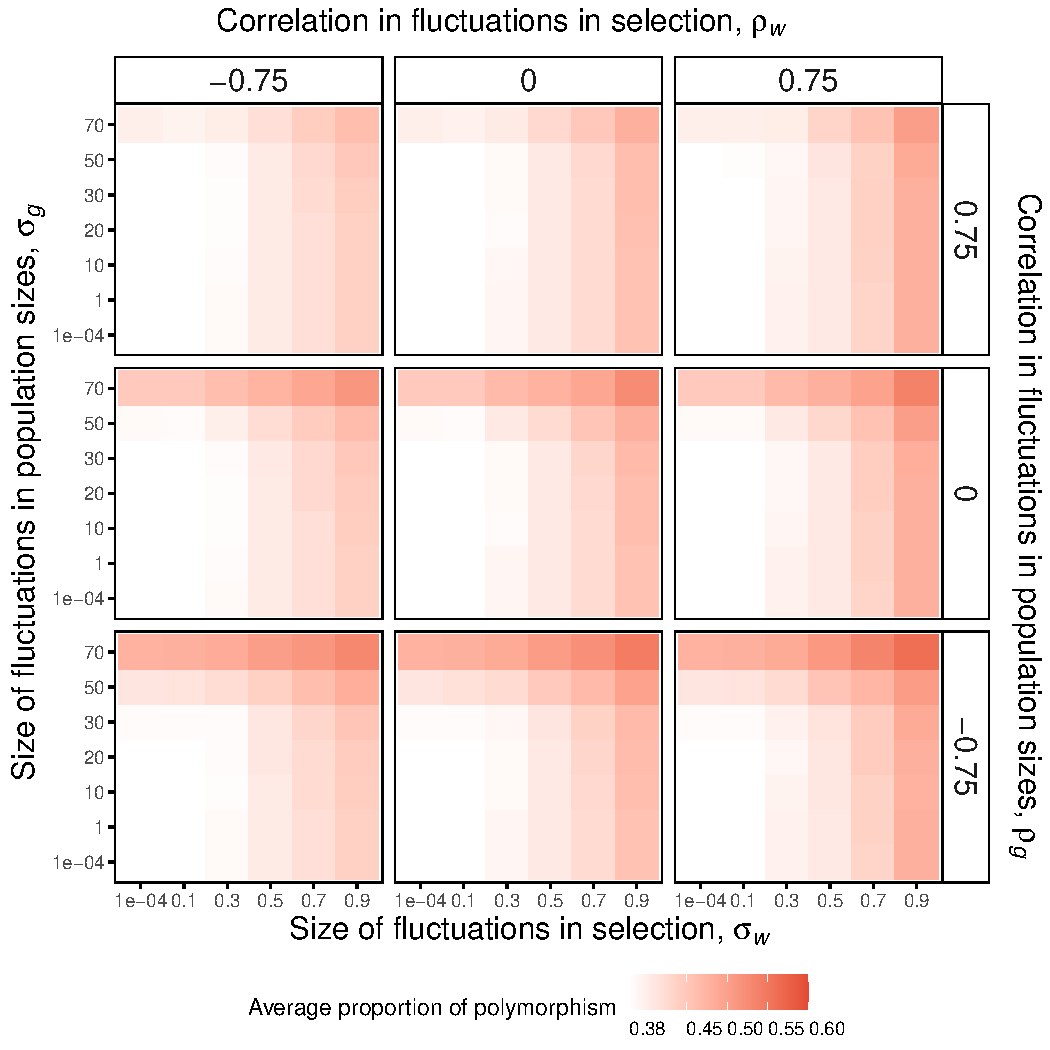
\includegraphics[width=1\textwidth]{figures/chapter4_fig1.pdf}}
  \caption[The average proportion of the selection parameter space corresponding to polymorphism.]{The average proportion of the selection parameter space corresponding to polymorphism. For all parameter combinations in our simulations, we show the average proportion of polymorphism in our grids, for all ten replicates and invasion scenarios (each allele invading a different sex). Each panel corresponds to a different combination of correlations between fluctuations and rows and columns within a pannel show the size of fluctuations in population sizes and in selection, respectively. Labels on top indicate the correlation between fluctuations in selection $\rho_{w}$, while labels on the right show the correlation in fluctuations between fluctuations in population sizes $\rho_{g}$.  As a basis of comparison, we show the expected proportion of polymorphism in constant environments ($ 0.38$) as white in our color scheme.  }
    \label{fig:heatmap}
\end{figure}


Our results matched previous findings that in constant environments, polymorphism can be maintained in $ \approx 38\%$ of the parameter space, which corresponds to the parameter space where balancing selection maintains a domain bounded by Eqn.~\ref{selection} (Fig.~\ref{fig:outcomes}A). Increases in polymorphism when population sizes fluctuated occurred near the limit of the domain of balancing selection and were particularly pronounced when selection against both alleles was weak (Fig.~\ref{fig:outcomes}B). When selection against either of the alleles was strong ($ S_{m}, S_{f}> 0.75 $), fluctuations in population sizes did not increase polymorphism compared to the control (Fig.~\ref{fig:outcomes}B). Similarly, increases in polymorphism when selection fluctuated also occurred near the limit of the domain of balancing selection; however, fluctuations in selection did not affect polymorphism when selection against both alleles was weak ($ S_{m}, S_{f}< 0.25 $) (Fig.~\ref{fig:outcomes}C). When both population sizes and selection fluctuated, increases in polymorphism occurred regardless of the strength of selection (Fig.~\ref{fig:outcomes}D).

The effect of fluctuations in population sizes and selection was not homogeneous across the parameter space. The values of $\delta^{0}$, which captured the difference between invader and resident growth rates when selection and population sizes were set to their mean, were close to zero near the limit of the domain of balancing selection (Fig.~\ref{fig:space}). In contrast, the rest of the $\delta$ values were generally stronger in magnitude near the limit of the domain of selection  (Fig.~\ref{fig:space}). Despite their similar patterns in the parameter space, the relative contribution of each type of fluctuation to the growth rate of alleles when rare depended on the allele and sex where the invasion took place (Fig.~\ref{fig:space}).

Fluctuations in population sizes of males and females facilitated polymorphism when alleles invaded via the fluctuating population (Fig.~\ref{fig:boxes}). In contrast, fluctuations in the population size of one sex made it more difficult for either allele to invade via the other sex (Fig.~\ref{fig:boxes}). For example, the relative contribution of fluctuations in the male population, $\delta^{N_{m}}$, was positive for both alleles when they invaded via males and negative when they invaded via females, regardless of the correlation between fluctuations (Fig.~\ref{fig:boxes}). The relative contribution of both populations fluctuating,  $\delta^{N_{m}N_{f}}$, was positive when fluctuations were negatively correlated, had a negligible effect when fluctuations were not correlated, and had a negative effect when fluctuations were positively correlated (Fig.~\ref{fig:boxes}).

In contrast, the relative contribution of fluctuations in selection depended on the allele that was the invader, regardless of the sex where invasion occurred (Fig.~\ref{fig:boxes_selection}). For example, $\delta^{w_{jm}}$ which captured the relative contribution of fluctuations in selection against $j$ in males, was always positive when allele $k$ invaded but had negligible effects when allele $j$ invaded (Fig.~\ref{fig:boxes_selection}). The relative contribution of fluctuations of both types of selection was negative when fluctuations were negatively correlated, had a negligible effect when fluctuations were not correlated, and had a positive effect when fluctuations were positively correlated (Fig.~\ref{fig:boxes_selection}).


\begin{figure}[H]
  \centerline{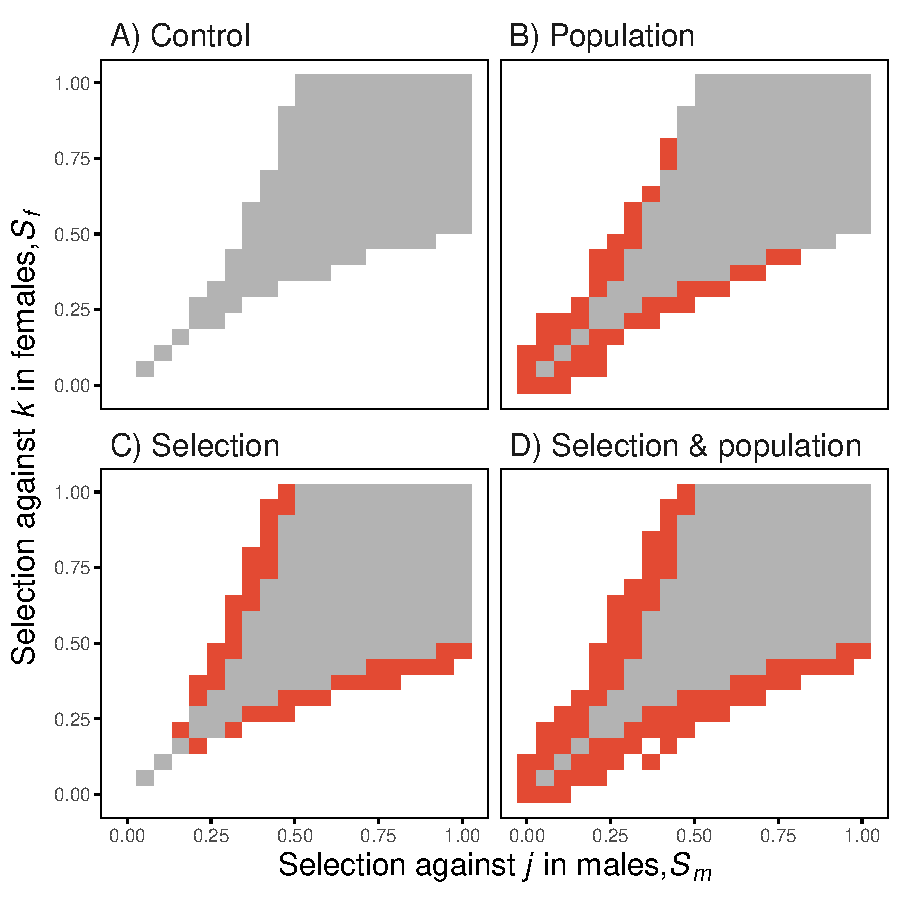
\includegraphics[width=1\textwidth]{figures/chapter4_fig2}}
  \caption[Polymorphism in the parameter space]{  Polymorphism in the parameter space. We show the outcomes of our invasion simulations  when $j$ invaded via males and $k$ invaded via females. As a reference, $j$ is favored in females and $k$ is favored in males. Each panel corresponds to a different replicate of our simulation grids. Grey areas indicate parts of the selection parameter space where polymorphism can be maintained without fluctuations while white areas indicate parts of the parameter space that correspond to the fixation of one of the alleles (following Eqn.\ref{selection}). Red areas indicate parts of the parameter space where polymorphism can be maintained when fluctuations were incorporated. In A) we show the outcomes of our control grid ($\sigma_{g}=0.0001$, $\rho_{g}=0$, $\sigma_{w}=0.0001$, $\rho_{w}=0$). In B) we show the outcomes when we incorporated high fluctuations in population sizes that were negatively correlated ($\sigma_{g}=70$, $\rho_{g}=-0.75$, $\sigma_{w}=0.001$, $\rho_{w}=0$). In C) we show the outcomes when we incorporated fluctuations in selection that were positively correlated  ($\sigma_{g}=0.0001$, $\rho_{g}=0$, $\sigma_{w}=0.9$, $\rho_{w}=0.75$). In D) we show the outcomes when both population sizes and selection fluctuated ($\sigma_{g}=70$, $\rho_{g}=-0.75$, $\sigma_{w}=0.9$, $\rho_{w}=0.75$). }
    \label{fig:outcomes}
\end{figure}

\begin{figure}[H]
  \centerline{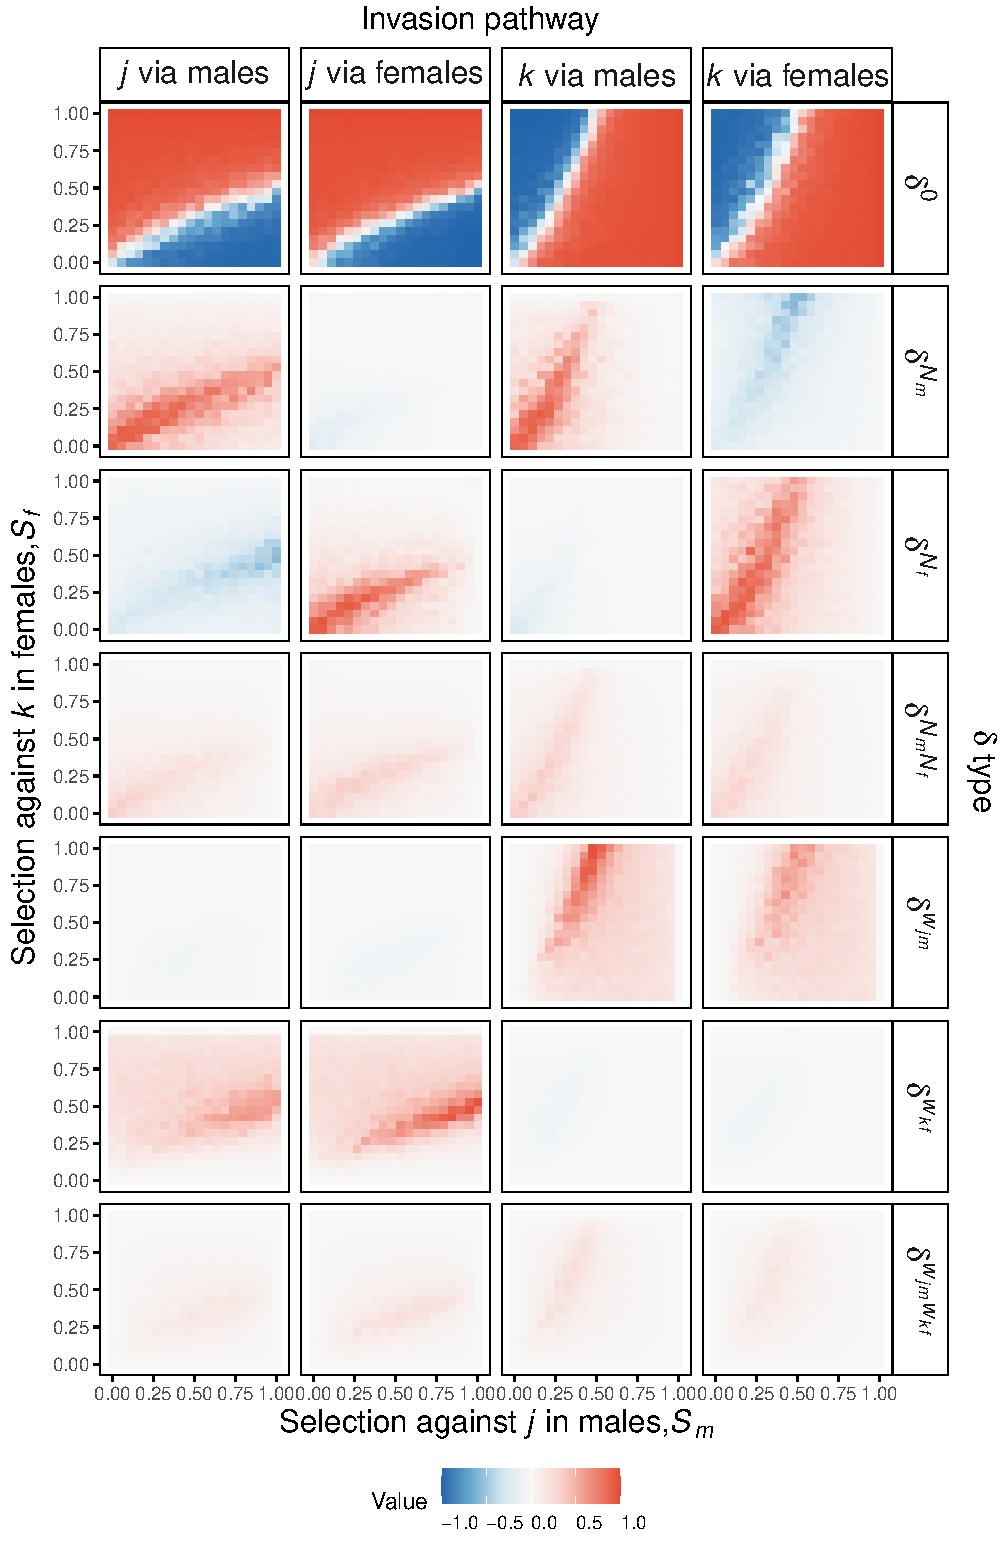
\includegraphics[width=1\textwidth]{figures/chapter4_fig3}}
  \caption[Distribution of $\delta$ values across the parameter space]{Distribution of $\delta$ values across the parameter space. We show the results of the functional decomposition approach for one replicate of our simulation grids where  both population sizes and selection fluctuated with correlated effects  ($\sigma_{g}=70$, $\rho_{g}=-0.75$, $\sigma_{w}=0.9$, $\rho_{w}=0.75$). Each row corresponds to a different type of $\delta$ value, as indicated with labels on the right. Each column corresponds to an allele invading a different pathway, as indicated with labels on top. Areas in red correspond to $\delta$ values that contributed positively to each allele's invasion growth rate, while blue areas denote points in the parameter space where fluctuations had a negative contribution to invasion growth rates.   }
    \label{fig:space}
\end{figure}


\begin{figure}[H]
  \centerline{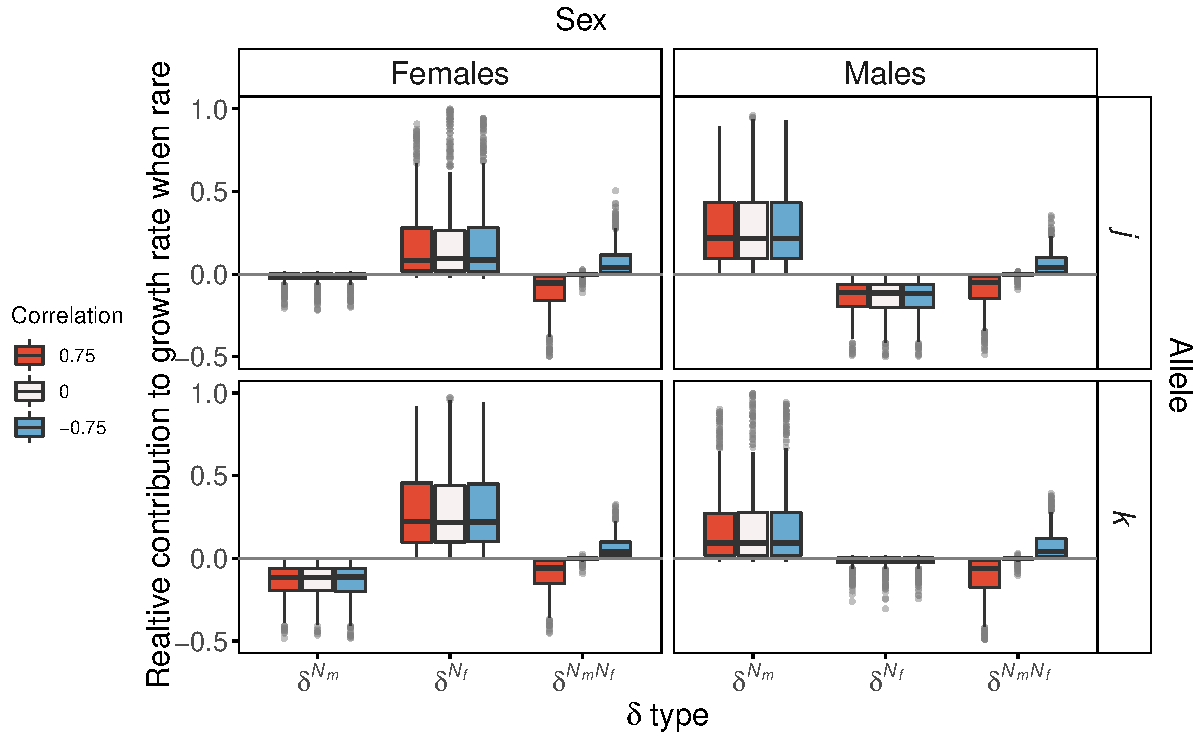
\includegraphics[width=1\textwidth]{figures/chapter4_fig4}}
  \caption[The relative contributions of fluctuations in population sizes to alleles' growth rates when rare]{The relative contributions of fluctuations in population sizes to alleles' growth rates when rare. Positive $\delta$ values imply that the corresponding fluctuation benefits that allele as an invader more than the other allele as a resident while negative $\delta$ values indicate fluctuations benefit the residents more than the invader. Each panel corresponds to the result of simulations where each allele invaded via a different pathway, as indicated by top and right labels. We show the boxplots of the three distinct $\delta$ values that captured the effects of fluctuations in population sizes, for all of the replicates in our simulation in which $\sigma_{g}=70$. Each color corresponds to a different correlation between fluctuations in population sizes ($\rho_{g}$), as the legend indicates. Box plots extend from the first to third quantiles of the corresponding $\delta$ values, and the line inside the the box indicates the median. The upper whisker extends to the largest value no further than 1.5 times the inter-quantile range (IQR, or the distance between the first and third quartiles); the lower whisker extends to the smallest value at most 1.5 times the IQR. Data beyond the end of the whiskers are determined to be outliers and are plotted individually with solid grey points. }
    \label{fig:boxes}
\end{figure}



\begin{figure}[H]
  \centerline{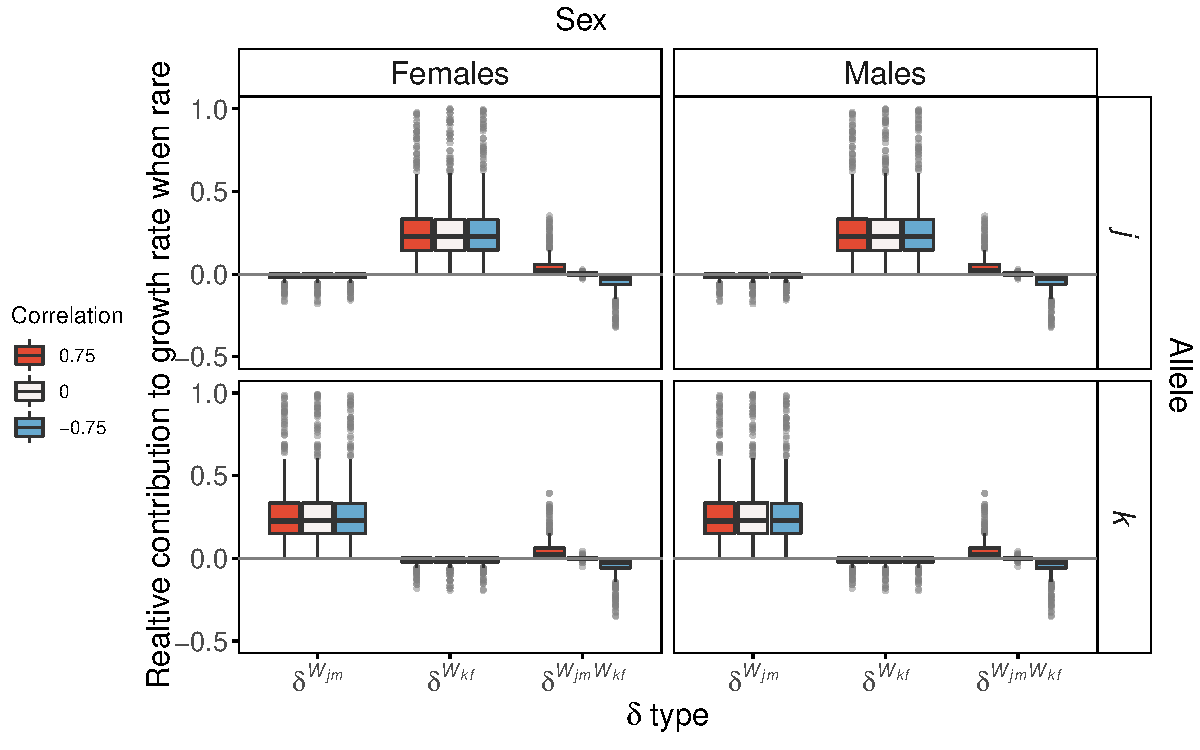
\includegraphics[width=1\textwidth]{figures/chapter4_fig5}}
  \caption[The relative contributions of fluctuations in selection to alleles' growth rates when rare.]{The relative contributions of fluctuations in selection to alleles' growth rates when rare. Positive $\delta$ values imply that the corresponding fluctuation benefits that allele as an invader more than the other allele as a resident while negative $\delta$ values indicate fluctuations benefit the residents more than the invader. Each panel corresponds to the result of simulations where each allele invaded via a different pathway, as indicated by top and right labels. We show the boxplots of the three distinct $\delta$ values that captured the effects of fluctuations in selection, for all of the replicates in our simulation in which $\sigma_{w}=0.9$. Each color corresponds to a different correlation between fluctuations in population sizes ($\rho_{w}$), as the legend indicates. Box plots extend from the first to third quantiles of the corresponding $\delta$ values, and the line inside the the box indicates the median. The upper whisker extends to the largest value no further than 1.5 times the inter-quantile range (IQR, or the distance between the first and third quartiles); the lower whisker extends to the smallest value at most 1.5 times the IQR. Data beyond the end of the whiskers are determined to be outliers and are plotted individually with solid grey points. }
    \label{fig:boxes_selection}
\end{figure}

\section*{Discussion}


The results of our study provide supporting evidence that environmental fluctuations can substantially increase the expected genetic variance maintained under sexually antagonistic selection (Fig.~\ref{fig:heatmap}). Perhaps more importantly, our study shows \textit{how} environmental fluctuations help maintain polymorphism by quantifying the relative contribution of fluctuations to alleles growth rates when rare. Antagonistically selected alleles are an important component of genetic variation for many species \citep{foerster2007sexually,van2009intralocus,bonduriansky2009intralocus,innocenti2010sexually}. Indeed, as much as $20\%$ of traits for which data are available are thought to be under sexually antagonistic selection \citep{morrissey2016meta}. Yet, a large body of work suggests that the criteria for maintaining antagonistic genetic variation are very restrictive (i.e., we would expect polymorphism to be maintained in a population in few scenarios) \citep{kidwell1977regions,pamilo1979genic,hedrick1999antagonistic,curtsinger1994antagonistic,patten2010fitness}. In contrast, our study shows that when we incorporated more realistic assumptions, a sexually antagonistic polymorphism can be maintained in up to $60\%$ of the parameter space (Fig.~\ref{fig:heatmap}).


\subsection*{The relative contribution of fluctuations in selection}


Our simulations indicate that large fluctuations in the strength of selection can substantially increase the proportion of polymorphism compared to when selection is constant (Fig.~\ref{fig:heatmap}). The effect of fluctuations in selection was generally greater in magnitude near the limit of the domain of selection and where selection against alleles was strong (Fig.~\ref{fig:space}). In contrast, fluctuations in selection had a minor effect when both alleles had similar fitness, suggesting that fluctuations in selection become advantageous when there exist greater fitness differences between sexually antagonistic alleles (Fig.~\ref{fig:space}). The effect of fluctuations in selection depended on the identity of the invading allele, regardless of the sex where invasion occurred (Fig.~\ref{fig:boxes_selection}). Our results suggest that in parts of the parameter space where one would expect selection to fix the allele with higher fitness, the allele with lower fitness can be maintained in a population if the fitter allele experiences high fluctuations in selection (Fig.~\ref{fig:outcomes}). This could be the case, for example, if traits associated with sexual dimorphism like ornaments or bright colors are also associated with higher predator rates \citep{bildstein1989consequences,gotmark1997natural} or sex-biased mortality \citep{promislow1992mortality}. However, if the allele with lower fitness is the one associated with higher fluctuations in selection, then fluctuations are not likely to promote the maintenance of both alleles in a population (Fig.~\ref{fig:boxes_selection}).


An exact correspondence with Modern Coexistence Theory is unlikely to be achieved when using the functional decomposition approach \citep{ellner2016quantify,shoemaker2020}. Similarly, when comparing evolutionary dynamics to competitive dynamics, the interpretation of coexistence mechanisms is not straightforward. Nonetheless, our quantification of the relative contributions of fluctuations to alleles' invasion growth rates show similarities to fluctuation dependent coexistence mechanisms. For example, the relative contributions of fluctuations in selection (captured by $\delta^{w_{jm}}$ and $\delta^{w_{kf}}$) is similar to the expected contributions to growth rates made by \textit{relative non-linearity}. This fluctuation dependent mechanism requires that competitors differ in the degree of non-linear responses to limiting competitive factors \citep{chesson2000mechanisms,chesson2003quantifying,zepeda2019fluctuation}. If differences in response to limiting factors exist, and the limiting factors fluctuate, non-linear averaging can benefit some species and hurt others \citep{ellner_expanded_2019}. In our model, fluctuations in selection against one allele affect both alleles differently (e.g., fluctuations in the fitness of allele \textit{j} in males affect both allele $j$ and $k$ to different extents). Thus, when selection against one allele fluctuated, it contributed positively to the growth rate of the other allele as an invader (Fig.~\ref{fig:boxes_selection}).


The interactive effect of fluctuations in selection, $\delta^{w_{jm},w_{kf}}$, promoted allelic coexistence when fluctuations were positively correlated, and it contributed negatively to each allele's invasion growth rate if fluctuations were negatively correlated (Fig.~\ref{fig:boxes_selection}). Environmental fluctuations are often correlated \citep{steele1985comparison}. Previous studies have shown that positively correlated environmental fluctuations can increase the invasion growth rate of a species when there are species-specific environmental responses, and there is buffered population growth where species are shielded from competition \citep{schreiber2021positively,chesson2000mechanisms}. This coexistence mechanism is known as the \textit{storage effect}, and it is often quantified as the contribution to an invasion growth rate of covariance between the environment and competitive factors \citep{ellner2016quantify,zepeda2019fluctuation}. In our model, fluctuations in $w_{jm}$ and $w_{kf}$ are not easily separated into environmental and competitive factors, therefore referring to this type of contribution as a storage effect would be misleading. Nonetheless, our results show that there exists a benefit when both $w_{jm}$ and $w_{kf}$ vary, beyond the contribution of each effect varying on its own when fluctuations are positively correlated. This could arise, for example, in environments where sexual selection on both sexes is stronger when climatic conditions are favorable and becomes negligible in stressful conditions \citep{cockburn2008swingin}.

\subsection*{The relative contribution of fluctuations in population sizes}

 Fluctuations in population sizes caused overall increases in the proportion of coexistence compared to the control simulation  (Fig.~\ref{fig:heatmap}).  The effect of fluctuations in population sizes was generally greater in magnitude near the limit of the domain of selection where both alleles had similar fitness values and had a weaker effect as differences in fitness were larger (Fig.~\ref{fig:space}). This suggests that fluctuations in population sizes will likely play a minor role in maintaining polymorphism in populations where sexual antagonism is strong.  Similar to fluctuations in selection, fluctuations in population sizes had positive contributions to the invasion growth rate of alleles due to a mechanism similar to \textit{relative non-linearity}. Fluctuations in the population sizes of males and females had different effects on each allele. They thus, contributed positively to invasion growth rates if alleles invaded via the fluctuating population (Fig.~\ref{fig:boxes}). If an allele invaded via the non-fluctuating sex, however, fluctuations contributed negatively to its invasion growth rate and thus hampered the maintenance of polymorphism (Fig.~\ref{fig:boxes}).

 Our results suggest that in parts of the parameter space where we would expect selection to fix the allele with higher fitness the allele with lower fitness could achieve a positive invasion growth rate if it invaded via a population experiencing temporal changes in its size.  Temporal changes in population sizes of males and females can arise due to sex differences in movement \citep[e.g., if males immigrate to higher quality areas;][]{matter2002experimental}, development \citep[e.g., females requiring more time to mature than males;][]{kasumovic2008spatial}, and behavior \citep[e.g., cannibalistic mating;][]{elgar2003male}. When males and females experience different population dynamics, sexual antagonism allows alleles to respond differently to fluctuations and thus promotes the maintenance of polymorphism. The interactive effect of fluctuations in males and females, $\delta^{N_{m},N_{f}}$, shows that, when both populations fluctuate, negatively correlated fluctuations promote the maintenance of genetic diversity while positively correlated fluctuations likely impair it  (Fig.~\ref{fig:boxes}). These insights offer an exciting avenue of research to understand if sexually selected traits are more often found in populations that experience negatively correlated temporal changes in population sizes, and could help explain the high heritabilities of those traits \citep{reinhold2000maintenance}.

 \subsection*{Polymorphism and sexual conflict}

 Our study exclusively focused on the conditions for maintaining polymorphism in a population with and without environmental fluctuations. However, maintaining non-advantageous alleles in a population is costly and can result in a decrease in the overall fitness of a population \citep{gavrilets2014sexual,connallon2018environmental}. Sexually antagonistic selection necessarily creates a mismatch between the traits a population expresses and the optimal expression of those traits \citep{lande1980sexual}. It is often resolved once members of both sexes express traits that match the sex-specific optima (e.g., when alleles with lower fitness are eliminated from a population, the evolution of sex chromosomes or sex-specific expression of traits)\citep{lande1980sexual, arnqvist2013sexual}. Our results show that large fluctuations in selection and population sizes can impede the resolution of sexual conflict by maintaining multiple alleles in a population, even when selection against some of those alleles is strong (Fig.~\ref{fig:outcomes}D). Thus, the maintenance of genetic diversity promoted by fluctuations might involve strong trade-offs in the fitness and evolution of a population. These trade-offs can, in turn, result in an erosion of genetic diversity even when fluctuations are present.


 \subsection*{Conclusion}
Our study contributes to the growing body of work that shows that the usual criteria for maintaining genetic variation under sexually antagonistic selection are overly conservative \citep{connallon2012general,connallon_evolutionary_2019}. Processes like recurrent mutations \citep{radwan_maintenance_2008}, genetic drift \citep{connallon2012general}, local adaptations \citep{connallon_evolutionary_2019}, and alleles that experience seasonal changes in dominance \citep{wittmann2017seasonally} have all been shown to dramatically change the levels of sexually antagonistic variance in natural populations. Our results show that non-constant environments might promote the maintenance of genetic diversity of sexually antagonistic alleles without the need for local adaptations or life-history stages that involve overlapping generations. The environmental drivers that maintain sexually antagonistic traits are still poorly understood \citep{connallon2018environmental}. Our study provides a necessary precursor to fully characterize the effect of environmental drivers on genetic diversity by explicitly quantifying the contribution of environmental fluctuations to the maintenance of polymorphism across the selection parameter space.

\printbibliography
\end{refsection}
